\documentclass[11pt]{article}

% Change "review" to "final" to generate the final (camera-ready) version.
\PassOptionsToPackage{table}{xcolor}
\usepackage[review]{acl}

\usepackage{times}
\usepackage{latexsym}
\usepackage[T1]{fontenc}
\usepackage[utf8]{inputenc}
\usepackage{microtype}
\usepackage{inconsolata}
\usepackage{graphicx}
\graphicspath{{./}{figures/}}
\usepackage{booktabs}
\usepackage{amsmath}
\usepackage{algorithm}
\usepackage{algpseudocode}
\usepackage[skins,breakable]{tcolorbox}
\usepackage{placeins}

% Let wide floats sit near their first reference instead of drifting to the end.
\renewcommand{\topfraction}{0.95}
\renewcommand{\dbltopfraction}{0.95}
\renewcommand{\textfraction}{0.05}
\renewcommand{\floatpagefraction}{0.8}
\renewcommand{\dblfloatpagefraction}{0.8}
\setcounter{topnumber}{3}
\setcounter{dbltopnumber}{3}

% Palette: light blue and light green.
\definecolor{softblue}{HTML}{EAF3FC}
\definecolor{midblue}{HTML}{D3E5F6}
\definecolor{deepblue}{HTML}{1F5F99}
\definecolor{softgreen}{HTML}{E8F6EE}
\definecolor{midgreen}{HTML}{CFEBDA}
\definecolor{deepgreen}{HTML}{1F7A4A}
\definecolor{softred}{HTML}{FBE3E1}
\newtcolorbox{findingbox}{enhanced,breakable,colback=softgreen,colframe=deepgreen,boxrule=0.4pt,
  leftrule=2.2pt,arc=1.5pt,left=4pt,right=4pt,top=2pt,bottom=2pt,fontupper=\small}
\newcommand{\finding}{\begingroup\def\findingbody##1\par{\begin{findingbox}\textbf{\textcolor{deepgreen}{Finding.}} ##1\end{findingbox}\endgroup}\findingbody}
\newtcolorbox{promptbox}[2][]{enhanced,breakable,colback=#2!40,colframe=#2!70!black,boxrule=0.5pt,
  arc=2pt,left=5pt,right=5pt,top=3pt,bottom=3pt,fontupper=\footnotesize,#1}

\title{What Did the Prompt Edit Break? Item-Level Regression Tracking\texorpdfstring{\\}{ }for Automatic Prompt Optimization}

% Submissions must be fully anonymous.
\author{Anonymous submission}

\begin{document}
\maketitle

\begin{abstract}
Teams that maintain LLM prompts need to know which inputs a revision fixes and which it breaks, yet automatic prompt optimization (APO) is usually judged by aggregate accuracy alone. Motivated by this problem in an industrial document-processing pipeline, we built Reflective Feedback-Driven Prompt Optimization (RFDPO), an auditable optimizer that records, for every revision, the items it recovers (wrong to right) and regresses (right to wrong), and returns this effect report to the optimizer. RFDPO is not yet deployed, so we evaluate it on five public benchmarks covering law, knowledge, instruction following, mathematics, and privacy, with GPT-5 as optimizer and GPT-4o-mini and GPT-4.1 Mini as solvers. Aggregate accuracy hid much of what changed: in five of nine configurations, the number of test items that changed correctness was at least five times the net change, and a one-item net change hid up to 17 changed items. Mean test gains were 66\% of mean validation gains (5.2 vs.\ 7.9 points), and nearly all net mining-set progress came in the first round. In a controlled ablation, the effect report and its accompanying instructions made revisions more conservative, with fewer changed and fewer regressed items, but did not improve accuracy. We turn these results into practical lessons for reviewing and reporting prompt changes.
\end{abstract}

\section{Introduction}
\label{sec:intro}

\begin{figure*}[!t]
\centering
\includegraphics[width=\textwidth]{fdpo2.png}
\caption{The RFDPO loop. The solver evaluates prompts on mining set $M$ and validation set $V$. From the second round,
the optimizer receives the item-level effect of its previous edit before proposing a new prompt. Every changed
candidate is committed, and RFDPO returns the candidate with the highest validation accuracy, breaking ties by mining
accuracy and then by the earlier round (eight runs used an earlier final-round rule; \S\ref{sec:method}). Test set $T$
is excluded from feedback and selection and evaluated only for the seed and the returned prompt.}
\label{fig:arch}
\end{figure*}

Prompts in deployed LLM applications are maintained like code: they are revised when a new input type fails, a model version changes, or an output format must be tightened. Each revision changes a shared component, and in machine-learning systems such changes rarely stay local~\citep{sculley2015debt}. Engineers who build LLM products describe prompt revision as trial and error and name testing as a main difficulty~\citep{parnin2023copilot}. In open-source repositories, only 21.9\% of 1,262 observed prompt changes were documented in commit messages~\citep{tafreshipour2025prompting}. The same hosted model can also change behavior between versions~\citep{chen2023drift} and between repeated runs at fixed settings~\citep{atil2025nondeterminism}.

This work began with that problem in an industrial document-processing pipeline, where LLM prompts extract fields from scanned documents. Revisions that fixed one class of documents could change answers, or break the required output format, on documents that had been processed correctly; practitioners who depend on structured output report the same concern~\citep{liu2024structured}. An aggregate score showed whether a revision helped on balance, but not which documents it fixed and which it broke. Automatic prompt optimization (APO), in which an optimizer LLM revises the prompt of a solver LLM from evaluation feedback~\citep{zhou2023ape,yang2024opro,pryzant2023protegi}, has the same blind spot: methods are compared by accuracy before and after optimization. For hosted-model updates, \citet{ma2024regression} found that previously correct predictions broke in 87.9\% of cases where aggregate accuracy improved. A prompt optimizer that ships a revision faces the same risk.

Two revisions that each gain two items can differ: one recovers two items and breaks none, while another recovers ten and breaks eight. To make this difference visible, we built \emph{Reflective Feedback-Driven Prompt Optimization} (RFDPO; Figure~\ref{fig:arch}). RFDPO compares every revision with its parent item by item, records \emph{recoveries} (incorrect to correct), \emph{regressions} (correct to incorrect), and \emph{churn} (their sum), and returns this effect report to the optimizer in the next round. It keeps every prompt version with its outcomes and cost, so each change can be audited. RFDPO has not yet been deployed in the pipeline that motivated it. Because those documents cannot be released, we evaluate it on five public benchmarks with two low-cost hosted solvers, so the results can be reproduced. Our contributions are:

\begin{itemize}
\setlength{\itemsep}{1pt}
\setlength{\parskip}{0pt}
\setlength{\topsep}{1pt}

\item \textbf{An auditable optimizer.} RFDPO records item-level transitions for every revision and feeds them back to the optimizer (\S\ref{sec:method}).

\item \textbf{Evidence that aggregate accuracy hides churn.} In five of nine configurations, test churn was at least five times the net change, and a one-item net change hid up to 17 changed items (\S\ref{sec:itemresults}).

\item \textbf{Evidence on transfer and round budget.} Test gains were 66\% of validation gains, and nearly all net tuning progress came in round~1 (\S\ref{sec:valtest}, \S\ref{sec:rounds}).

\item \textbf{A negative result on feedback.} In a controlled ablation, the effect report and its instructions reduced churn and regressions but did not improve accuracy (\S\ref{sec:ablation}).

\end{itemize}

\noindent We close with lessons for teams that review prompt changes (\S\ref{sec:lessons}).

\section{Related Work}
\label{sec:related}

\paragraph{Automatic prompt optimization.}
APO methods search over instructions with LLM proposals~\citep{zhou2023ape,yang2024opro}, textual gradients~\citep{pryzant2023protegi,yuksekgonul2025textgrad}, evolutionary search~\citep{guo2024evoprompt,fernando2024promptbreeder}, or pipeline-level optimization~\citep{opsahlong2024miprov2,schnabel2024sammo,khattab2024dspy}; earlier work searched discrete tokens~\citep{shin2020autoprompt}. MPO~\citep{sharma2026mpo} uses the five-section prompt structure that RFDPO adopts. GEPA~\citep{agrawal2026gepa} reflects on execution traces and selects candidates on a Pareto front, Trace2Policy~\citep{zha2026trace2policy} clusters errors and gates refinements on regressions, and self-feedback methods revise from verbal critiques~\citep{madaan2023selfrefine,shinn2023reflexion}. RFDPO differs in what it feeds back: the item-level consequences of the previous edit, including the items it broke. It has no regression gate, so its record keeps every change, including harmful ones.

\paragraph{Regressions and consistency.}
Aggregate accuracy hides behavioral change~\citep{ribeiro2020checklist}; negative flips motivated regression-free model updates~\citep{yan2021positive}, and paired comparison of outcomes goes back to \citet{mcnemar1947sampling}. In LLM applications, regressions arise from model updates~\citep{ma2024regression,chen2023drift}, small prompt changes~\citep{salinas2024butterfly,sclar2024quantifying,errica2025wrong}, and nondeterminism at fixed settings~\citep{atil2025nondeterminism}, although some apparent sensitivity is an evaluation artifact~\citep{hua2025flaw}. We apply this regression view to successive revisions within prompt optimization.

\paragraph{Evaluation protocols.}
Published APO results differ in splits, solvers, baselines, and feedback, so their scores are not directly comparable (Appendix~\ref{app:prior}). Tuning gains may not transfer to new data~\citep{recht2019imagenet}, and contamination is a further risk~\citep{oren2023proving}. In a diagnostic run, supplying test items as optimizer feedback raised Hearsay accuracy to 95.3\%, against 73.4\% with the items held out (Appendix~\ref{app:oracle}). RFDPO therefore keeps test items out of feedback and selection.



\section{RFDPO}
\label{sec:method}

\paragraph{Prompts and data.}
A solver LLM executes the task and an optimizer LLM revises the solver's prompt; no model weights change. Following MPO~\citep{sharma2026mpo}, every prompt has five fixed sections (System Role, Context, Task Details, Constraints, Output Format), so each revision can be traced to the sections it changed. RFDPO uses three disjoint sets. The mining set $M$ supplies failures and successes to the optimizer. The validation set $V$ selects the returned prompt and, from round~2, also appears in the feedback. The test set $T$ is evaluated only for the seed and the returned prompt and never enters feedback or selection.

\paragraph{Item-level transitions.}
\label{sec:metric}
Let $c_i(p)\in\{0,1\}$ be the observed correctness of item $i$ under prompt $p$. For prompts $p$ and $q$ evaluated on the same items $D$, the recovered and regressed sets are
\begin{equation*}
\begin{aligned}
R&=\{i\in D:c_i(p)=0,\ c_i(q)=1\},\\
G&=\{i\in D:c_i(p)=1,\ c_i(q)=0\}.
\end{aligned}
\end{equation*}
The net change $N=|R|-|G|$ equals $|D|$ times the accuracy difference, and churn is $C=|R|+|G|$. Churn counts changes in correctness only: an answer that changes from one wrong value to another wrong value is not counted, nor is a free-text output that changes but still fails. On test, this leaves out 9 AIME items and 23 MMLU items whose wrong answer changed (Appendix~\ref{app:eval}). Transitions are computed between consecutive committed prompts on $M$ and $V$, and between the seed and the returned prompt on $T$, over items evaluated under both prompts (Figure~\ref{fig:metric} in Appendix~\ref{app:algorithm}).

\paragraph{Effect-report feedback.}
\label{sec:optimization}
In each round the optimizer receives the current prompt, every mining failure with the solver's answer and the gold answer, and every mining success. From round~2 it also receives the \emph{effect report} of its previous revision: the previous text of each changed section, every recovered and regressed item on $M$ and $V$ (with the new wrong output for regressions), and the change in validation accuracy. Its system prompt asks it to keep edits linked to recoveries, repair edits linked to regressions, and leave unimplicated wording alone (Appendix~\ref{app:sysprompt}). The report shows co-occurrence, not causation: when a revision changes several sections, it cannot say which change moved which item, and some movement can be re-evaluation noise (Appendix~\ref{app:noise}). Every changed candidate is committed as the next parent, even if validation accuracy falls; there is no regression gate. RFDPO logs every prompt version, changed section, item outcome, and token cost (Algorithm~\ref{alg:reflect} in Appendix~\ref{app:algorithm}).

\paragraph{Selection rule.}
\label{sec:selection}
RFDPO returns the committed candidate with the highest validation accuracy, breaking ties by mining accuracy and then by the earlier round; the seed is returned only if no candidate is committed. We adopted this rule after the GPT-4o-mini PUPA run showed its round~2 ahead of the final round~3 on both mining (86.2\% vs.\ 82.8\%) and validation (63.3\% vs.\ 53.3\%). Eight of the 19 runs reported here, the GPT-4o-mini runs on PUPA, IFBench, and the six MMLU subjects, had already finished under the earlier rule, which returned the final round, and their optimizer had been told that the final round would ship. We report them as recorded: reselecting a round afterwards would not reproduce a run whose optimizer had been given the best-validation rule. Section~\ref{sec:valtest} quantifies the effect of this difference.

\section{Experimental Setup}
\label{sec:setup}

\paragraph{Benchmarks.}
Table~\ref{tab:setup} lists the five benchmarks and the split sizes actually evaluated. \textbf{LegalBench-Hearsay}~\citep{guha2023legalbench} is binary classification under U.S.\ hearsay law. \textbf{MMLU}~\citep{hendrycks2021mmlu} contributes six four-way multiple-choice subjects (college mathematics, computer security, econometrics, high-school biology, philosophy, professional law), each optimized separately and macro-averaged. \textbf{IFBench}~\citep{pyatkin2025ifbench} checks verifiable output constraints with a programmatic verifier in the style of IFEval~\citep{zhou2023ifeval}; an item is correct only if every constraint holds. \textbf{AIME}~\citep{maa2025aime} uses the 2022--2024 problems for optimization and the 30 problems of 2025 for test. \textbf{PUPA}~\citep{li2025papillon} measures privacy-conscious delegation: the optimized prompt rewrites a private query before it is sent to an external model. Each PUPA item receives a composite score $(\mathrm{quality}+1-\mathrm{leakage})/2$. We report PUPA \emph{accuracy}, the share of items with composite score $\geq 0.7$; mean composite scores, the metric reported by GEPA, appear only in Appendix~\ref{app:prior}.

\begin{table}[!t]
\centering
\small
\setlength{\tabcolsep}{4pt}
\begin{tabular}{llc}
\toprule
\rowcolor{midblue}
Benchmark & Task & $M$/$V$/$T$ evaluated \\
\midrule
Hearsay & Binary classification & 25/25/49 \\
MMLU (6 subj.) & Multiple choice & 25/25/66$^{a}$ \\
IFBench & Instruction following & 20/19/42$^{b}$ \\
 & & 25/14/42$^{b}$ \\
AIME & Integer answer & 58/32/30 \\
PUPA & Private-query rewriting & 29/30/38$^{c}$ \\
\bottomrule
\end{tabular}
\caption{Evaluated split sizes, identical for both solvers unless noted. Differences from the assigned sizes are items blocked by the provider's content filter, which we exclude rather than score as wrong. $^{a}$Per subject; professional law 25/22/63. $^{b}$GPT-4o-mini (assigned 20/20/42) and GPT-4.1 Mini (assigned 26/14/42). $^{c}$Assigned 30/30/40.}
\label{tab:setup}
\end{table}

\paragraph{Models and protocol.}
The solvers are GPT-4o-mini~\citep{openai2024gpt4o} and GPT-4.1 Mini~\citep{openai2025gpt41}, two low-cost hosted models, at temperature~0; the optimizer is GPT-5~\citep{openai2025gpt5} at temperature~0.7. PUPA also uses a fixed GPT-4.1 external model and a GPT-5 quality judge. Each run uses seed~0 and at most three rounds with one optimizer call per round, and optimization is skipped when seed mining accuracy reaches 95\% (except on PUPA). This gives 19 matched seed/returned records: seven non-MMLU runs and twelve MMLU subject runs. The two IFBench runs used different validation fractions (0.50 and 0.35). Two earlier AIME runs with a 2,048-token output limit are reported only in Appendix~\ref{app:aime_extra}. Settings, scoring, and optimizer prompts are in Appendices~\ref{app:config}--\ref{app:prompts}.

\section{Findings}
\label{sec:results}

\subsection{Aggregate accuracy hides churn}
\label{sec:itemresults}

\begin{table*}[!t]
\centering
\small
\setlength{\tabcolsep}{4pt}
\begin{tabular}{llrrrrrrr}
\toprule
\rowcolor{midblue}
 &  & \multicolumn{3}{c}{Test accuracy (\%)} & &
\multicolumn{3}{c}{Test transitions} \\
\cmidrule(lr){3-5}\cmidrule(lr){7-9}
\rowcolor{midblue}
Benchmark & Solver & Seed & Returned & $\Delta T$ & $\Delta V$ & $|R|$ & $|G|$ & Churn (\%) \\
\midrule
AIME & GPT-4.1 Mini & 53.3 & 50.0 & $-3.3$ & $+6.2$ & 3 & 4 & 7 (23.3) \\
\rowcolor{softgreen}
PUPA & GPT-4o-mini$^\dagger$ & 55.3 & 65.8 & $+10.5$ & $+13.3$ & 7 & 3 & 10 (26.3) \\
\rowcolor{softgreen}
PUPA & GPT-4.1 Mini & 44.7 & 71.1 & $+26.3$ & $+23.3$ & 10 & 0 & 10 (26.3) \\
\rowcolor{softgreen}
IFBench & GPT-4o-mini$^\dagger$ & 40.5 & 45.2 & $+4.8$ & $+15.8$ & 6 & 4 & 10 (23.8) \\
\rowcolor{softgreen}
IFBench & GPT-4.1 Mini & 42.9 & 66.7 & $+23.8$ & $+14.3$ & 12 & 2 & 14 (33.3) \\
Hearsay & GPT-4o-mini & 71.4 & 69.4 & $-2.0$ & $+12.0$ & 8 & 9 & 17 (34.7) \\
\rowcolor{softgreen}
Hearsay & GPT-4.1 Mini & 71.4 & 73.5 & $+2.0$ & $+20.0$ & 7 & 6 & 13 (26.5) \\
\rowcolor{softgreen}
MMLU (macro) & GPT-4o-mini$^\dagger$ & 75.1 & 77.2 & $+2.0$ & $+5.5$ & 31 & 23 & 54 (13.7) \\
\rowcolor{softgreen}
MMLU (macro) & GPT-4.1 Mini & 81.0 & 83.3 & $+2.3$ & $-0.7$ & 17 & 8 & 25 (6.4) \\
\bottomrule
\end{tabular}
\caption{Seed and returned prompts on test, with the validation change $\Delta V$; changes are in percentage points, computed from unrounded accuracies. $|R|$ and $|G|$ count recovered and regressed test items; churn is $|R|+|G|$, with its share of evaluated test items. Green rows have positive $\Delta T$. PUPA accuracy is the share of items with composite score $\geq 0.7$ (not the mean composite of Appendix~\ref{app:prior}). MMLU accuracy is macro-averaged over six subjects, and its transitions are summed over 393 items. $^\dagger$Returned by the earlier final-round rule (\S\ref{sec:selection}).}
\label{tab:main}
\end{table*}

Table~\ref{tab:main} compares the seed and returned prompts on test. Test accuracy rose in seven of nine configurations, by up to 26.3 points (PUPA, GPT-4.1 Mini), but net change understates how much moved. On Hearsay, one-item net changes hid 13 and 17 changed items, 27--35\% of the test set. On MMLU with GPT-4o-mini, 54 items changed correctness for a net gain of eight. In five of nine configurations, churn was at least five times the absolute net change (Figure~\ref{fig:rr} in Appendix~\ref{app:gap}). For a team deciding whether to ship a revision, each of these items is an input whose handling changes with no sign of it in the headline score.

\subsection{Validation gains overstate test gains}
\label{sec:valtest}

\begin{table}[!t]
\centering
\small
\resizebox{\linewidth}{!}{
\begin{tabular}{lrrrrr}
\toprule
\rowcolor{midblue}
Edited-prompt returns & Runs & Val.\ $\uparrow$ &
\shortstack{Val.\ $\uparrow$\\test $\downarrow$} &
$\overline{\Delta V}$ & $\overline{\Delta T}$ \\
\midrule
Non-MMLU & 7 & 7 & 2 & $+15.0$ & $+8.9$ \\
MMLU subjects & 10 & 5 & 1 & $+2.9$ & $+2.6$ \\
\textbf{All matched} & \textbf{17} & \textbf{12} & \textbf{3} &
$\mathbf{+7.9}$ & $\mathbf{+5.2}$ \\
\bottomrule
\end{tabular}}
\caption{Mean validation and test changes (points) for the 17 runs that returned an edited prompt; the other two retained the seed. Runs are weighted equally. The fourth column counts runs whose validation accuracy rose while test accuracy fell.}
\label{tab:gap}
\end{table}

Of the 19 records, 17 returned an edited prompt. Validation accuracy rose in 12 of them, stayed equal in three, and fell in two. In three of the 12, test accuracy fell by one item: AIME with GPT-4.1 Mini ($+6.2$ validation, $-3.3$ test points), Hearsay with GPT-4o-mini ($+12.0$, $-2.0$), and MMLU computer security with GPT-4o-mini ($+8.0$, $-1.5$). On average, validation rose by 7.9 points and test by 5.2, so test gains were 66\% of validation gains (Table~\ref{tab:gap}); the gap was small on MMLU ($+2.9$ vs.\ $+2.6$) and large elsewhere ($+15.0$ vs.\ $+8.9$). Because validation items enter the feedback from round~2, validation accuracy is a tuning score, not an independent estimate. Returned prompts contained no verbatim copies of benchmark items beyond a generic mathematical phrase and a True/False answer pattern (Appendix~\ref{app:overlap}).

\paragraph{Effect of the selection rule.}
The eight final-round runs did not always return their best-validation round. In three of them (PUPA, IFBench, and MMLU professional law), the final round had lower validation accuracy than round~2; for example, PUPA fell from 63.3\% in round~2 to 53.3\% in round~3. Under the best-validation rule, five of the eight would have returned an earlier round: those three, plus two with equal validation accuracy (Table~\ref{tab:selection} in Appendix~\ref{app:selection}). Their mean validation gain would rise from $+7.8$ to $+11.6$ points, and that of all 17 edited returns from $+7.9$ to $+9.7$. Only one alternative round was evaluated on test: PUPA round~2 scored 63.2\%, against 65.8\% for the returned round~3, so its higher validation accuracy did not carry over. The reported validation gains are therefore lower than a uniform best-validation rule would give, and the 66\% ratio describes the rules as run; the ratio under a uniform rule would require test scores for the other alternative rounds, which we did not collect.

\subsection{Most net progress arrives in round 1}
\label{sec:rounds}
\label{sec:edits}

Pooled over the 17 optimized runs, round~1 recovered 59 mining items and regressed 27 (net $+32$), whereas rounds 2--3 together recovered 56 and regressed 54 (net $+2$). On validation, the net change was $+17$, $+14$, and $-8$ in rounds 1, 2, and 3. Round~1 changed 4.3 of the five sections on average, later rounds 1.3. The share of correct mining items that regressed stayed near 8\% (27/315 in round~1, 54/655 later), but the share of failing items recovered fell from 40\% to 25\% (59/149 vs.\ 56/222). Later rounds therefore mostly exchanged some correct items for others. Because the effect report is present only from round~2, these runs cannot separate the report from the round; the ablation below holds the round fixed. We did not evaluate intermediate rounds on test, so we cannot say whether later rounds helped or hurt on unseen data.

\subsection{What the effect report changes}
\label{sec:ablation}

To isolate the report, we ran a controlled ablation on Hearsay with GPT-4o-mini. Both arms replay the round-1 prompt of the main run and then run rounds 2 and 3, five times each. They differ only in whether the optimizer receives the effect report and the system-prompt instructions that refer to it (Appendix~\ref{app:ablation}).

\begin{table}[!t]
\centering
\small
\setlength{\tabcolsep}{3pt}
\begin{tabular}{lrrr}
\toprule
\rowcolor{midblue}
Mean per run & Report & No report & $p$ \\
\midrule
Changed items per round ($M{+}V$) & 7.2 & 11.4 & .024 \\
Regressions per round ($M{+}V$) & 1.9 & 4.3 & .048 \\
Net gain per round ($M{+}V$) & 3.4 & 2.8 & .675 \\
New mining flips, rounds 2--3 & 2.4 & 6.6 & .016 \\
Undoing mining flips, rounds 2--3 & 3.8 & 3.8 & 1.000 \\
Test change (points) & $-5.3$ & $-5.7$ & 1.000 \\
Test churn & 14.2 & 17.2 & .270 \\
\bottomrule
\end{tabular}
\caption{Effect-report ablation on Hearsay with GPT-4o-mini, five runs per arm. A \emph{new} flip changes a mining item that the previous round left unchanged; an \emph{undoing} flip reverses the previous round's flip. $p$: exact two-sided permutation test over runs, uncorrected for multiple comparisons. Per-round counts are in Appendix~\ref{app:ablation}.}
\label{tab:ablation}
\end{table}

With the report, fewer items changed correctness per round on $M$ and $V$ (7.2 vs.\ 11.4) and fewer regressed (1.9 vs.\ 4.3), at a similar net gain (3.4 vs.\ 2.8; Table~\ref{tab:ablation}). The difference lies in \emph{new} flips: flips that undid the previous round's flip were equally common in both arms (3.8 per run), whereas flips on items the previous round had left alone fell from 6.6 to 2.4 per run. Smaller edits do not explain this, since round-2 revisions changed 2.0 sections with the report and 1.6 without it. Test accuracy fell in both arms ($-5.3$ and $-5.7$ points), so the report made revisions more conservative, not better.

Two caveats limit the attribution. First, the no-report arm also loses the instruction ``Do not churn wording that was not implicated by the evidence'', so the effect belongs to the report together with its instructions; separating them requires a third arm, which we have not run. Second, the ablation covers one benchmark and one solver, with five runs per arm and uncorrected tests.

\subsection{Cost}
\label{sec:resources}

Each non-MMLU run used three optimizer calls and cost between \$0.21 (IFBench, GPT-4o-mini) and \$4.80 (PUPA, GPT-4.1 Mini) at logged prices, including seed and final evaluations; the six MMLU subjects together cost \$1.32 and \$1.10 (Table~\ref{tab:resources} in Appendix~\ref{app:resources}). Optimizer input ranged from 14K tokens (Hearsay, GPT-4.1 Mini) to 498K (AIME). Transition tracking itself adds no model calls: it reuses the per-item outcomes that any evaluation already produces.

\section{Lessons for Practitioners}
\label{sec:lessons}
\label{sec:discussion}

These results suggest five practices for teams that revise prompts in production, whether by hand or with an optimizer.

\begin{enumerate}
\setlength{\itemsep}{1pt}
\setlength{\parskip}{0pt}
\setlength{\topsep}{1pt}
\item \textbf{Review a prompt change like a code change, with an item-level diff.} Report recoveries and regressions next to the accuracy change. In five of nine configurations, churn was at least five times the net change, so a release check on accuracy alone would have missed most of what changed. Once per-item outcomes are logged, the diff costs nothing extra.
\item \textbf{Treat tuning scores as optimistic.} Test gains were two-thirds of validation gains, and validation items also fed the optimizer. Keep a sealed test set that neither people nor the optimizer see before the release decision; in our diagnostic, exposing test items as feedback raised Hearsay accuracy from 73.4\% to 95.3\%.
\item \textbf{Fix the selection rule before running, and report it.} Returning the final round instead of the best-validation round changed the returned prompt in five of eight runs.
\item \textbf{Budget few rounds and expect noise.} Nearly all net mining gain came in round~1, and later rounds mostly exchanged correct items. An unchanged prompt can also flip items on re-evaluation (Appendix~\ref{app:noise};~\citealp{atil2025nondeterminism}), so a few flips should be confirmed before they drive the next revision.
\item \textbf{Use effect feedback for stability, not accuracy.} The effect report and its instructions reduced new flips and regressions, which matters when downstream systems depend on stable outputs, but did not raise accuracy.
\end{enumerate}

\section{Conclusion}
Prompt revisions in deployed LLM systems should be judged by what they fix and what they break. RFDPO records both for every revision made during automatic prompt optimization and returns them to the optimizer. Across five public benchmarks and two solvers, aggregate accuracy hid much of the item-level change, test gains were two-thirds of validation gains, and nearly all net tuning progress came in the first round. The effect report made revisions more conservative but did not improve accuracy. The next step is to apply RFDPO to the document-processing pipeline that motivated it, with per-round test evaluation and repeated seeds.

\section*{Limitations}
\label{sec:limitations}

\paragraph{Not yet deployed.}
RFDPO was motivated by an industrial pipeline but has been evaluated only on public benchmarks. We make no claim about its behavior on production data, where inputs, output formats, and the cost of an error differ.

\paragraph{Scope and statistics.}
We use five benchmarks, two closed-weight solvers, one optimizer, a single seed, at most three rounds, and small splits (14 to 66 evaluated items per set). Intermediate rounds were not evaluated on test, so we cannot say whether later rounds help on unseen data.

\paragraph{Mixed selection rule.}
Eight GPT-4o-mini runs returned the final round rather than the best-validation round; under the best-validation rule, five of them would have returned a different round (\S\ref{sec:valtest}). Comparisons between the two solvers therefore also compare selection rules.

\paragraph{Ablation confound.}
The no-report arm removes both the effect report and the instructions that refer to it, including ``Do not churn wording that was not implicated by the evidence''. We cannot tell which of the two reduced churn. The ablation also covers one benchmark and one solver, with five runs per arm and uncorrected $p$-values.

\paragraph{Attribution within a revision.}
A revision can change several sections at once. We attribute transitions to the revision as a whole, not to a section or an individual edit, and some transitions reflect re-evaluation noise rather than the prompt change (Appendix~\ref{app:noise}). The worked examples in Appendix~\ref{app:evolution} are descriptive, not causal.

\paragraph{What churn counts.}
Churn counts changes in correctness only. A wrong answer that changes to a different wrong answer (9 AIME and 23 MMLU test items) is not counted, nor is a PUPA score change that stays on one side of the 0.7 threshold.

\paragraph{Evaluation and data exposure.}
PUPA relies on an LLM judge, and the IFBench verifier implements 32 of 83 constraint types. Provider-blocked items are excluded rather than scored as errors. Validation items enter both feedback and selection, which can inflate tuning gains. The verbatim-overlap check cannot detect paraphrased copying.


\section*{Ethical Considerations}
Data come from public benchmarks, resplit as described in Table~\ref{tab:setup}. PUPA contains personal information from
public user--LLM conversations. Hosted solver and optimizer APIs receive the original queries during evaluation and
feedback; redaction protects only the designated external model. String-matched leakage does not capture paraphrased or
inferred information. No data from the industrial pipeline that motivated this work were used. Released traces would
contain item IDs and outcomes only, without raw inputs, predictions, or gold text (Appendix~\ref{app:artifacts}).

\FloatBarrier
\bibliography{custom}

% ACL rule: appendices must stay two-column (single column only for math-heavy sections).
\appendix

\section{Run Configuration and Scoring}
\label{app:config}
\subsection{Analysis Population and Settings}
\label{app:population}
The analysis uses 19 completed records: seven non-MMLU runs and twelve independently optimized MMLU
subjects, taking the latest completed record within each fixed run group.

All recorded solvers use temperature 0.0 and the GPT-5 optimizer uses 0.7, with at most three rounds and one optimizer
call per round. Table~\ref{tab:config} gives the configured solver output limits and splits for both solvers.
The response ledgers identify GPT-4o-mini-2024-07-18, GPT-4.1-mini-2025-04-14, and GPT-5-2025-08-07; some entries retain
model aliases rather than dated identifiers. PUPA additionally uses GPT-4.1 as its fixed external model and GPT-5 as judge.

\begin{table*}[!tp]
\centering
\small
\setlength{\tabcolsep}{5pt}
\begin{tabular}{llcccl}
\toprule
\rowcolor{midblue}Benchmark & Solver & Assigned $M/V$ & Val.\ fraction & Solver limit & Selection \\
\midrule
AIME & 4.1 Mini & 58/32 & 0.35 & 16,000 & best validation \\
PUPA & 4o-mini & 30/30 & 0.50 & 2,048 & final round \\
PUPA & 4.1 Mini & 30/30 & 0.50 & 2,048 & best validation \\
IFBench & 4o-mini & 20/20 & 0.50 & 2,048 & final round \\
IFBench & 4.1 Mini & 26/14 & 0.35 & 4,096 & best validation \\
Hearsay & both & 25/25 & 0.50 & 2,048 & best validation \\
MMLU (per subject) & 4o-mini & 25/25 & 0.50 & 2,048 & final round \\
MMLU (per subject) & 4.1 Mini & 25/25 & 0.50 & 2,048 & best validation \\
\bottomrule
\end{tabular}
\caption{Recorded settings for the matched runs. Solver limit is the configured maximum output tokens, not observed
consumption. Assigned pools precede provider-block exclusions; evaluated sizes are in Table~\ref{tab:setup}. Actual
resource use is in Table~\ref{tab:resources}.}
\label{tab:config}
\end{table*}

\paragraph{Candidate handling.}
Every changed candidate is committed and becomes the next parent. Best-validation selection compares committed
candidates, breaking ties by mining accuracy and then retaining the earlier candidate; the seed is excluded once a
candidate commits. The eight runs marked ``final round'' finished before this rule was adopted (\S\ref{sec:selection};
Appendix~\ref{app:selection}). Optimization is skipped at seed mining accuracy $\geq 0.95$, except on PUPA. This
retained the seed for GPT-4.1 Mini college mathematics and biology. IFBench with GPT-4.1 Mini proposed no change in
round 2.

\subsection{Optimization Procedure and Transition Example}
\label{app:algorithm}
Algorithm~\ref{alg:reflect} gives the optimization loop, and Figure~\ref{fig:metric} illustrates the transition counts.

\begin{algorithm}[htbp]
\caption{RFDPO optimization with edit-effect feedback}
\label{alg:reflect}
\small
\begin{algorithmic}[1]
\Require seed $p_0$; disjoint $M,V,T$; $\textsc{Opt}$; $\textsc{Solve}$; round budget $B$
\State $s_0,v_0 \gets \textsc{Solve}(p_0,M),\ \textsc{Solve}(p_0,V)$
\State $\tau_0 \gets \textsc{Solve}(p_0,T)$ \Comment{baseline; measured only}
\State $\mathcal{H}\gets\emptyset$; $(p,s,v)\gets(p_0,s_0,v_0)$; $\rho\gets\emptyset$
\For{$t=1$ \textbf{to} $B$}
  \If{skip threshold reached, or no mining failures} \State \textbf{break} \EndIf
  \State $q\gets\textsc{Opt}(p,s,v,\rho)$ \Comment{mining items and feedback}
  \If{$q=p$} \State \textbf{continue} \EndIf
  \State $s',v'\gets\textsc{Solve}(q,M),\ \textsc{Solve}(q,V)$
  \State $\rho\gets((R,G)(s\!\to\!s'),(R,G)(v\!\to\!v'))$
  \State append $(q,s',v')$ to $\mathcal{H}$ \Comment{no regression gate}
  \State $(p,s,v)\gets(q,s',v')$
\EndFor
\State $p^*\gets p_0$ if $\mathcal{H}=\emptyset$; otherwise select from $\mathcal{H}$
\Statex \hspace{\algorithmicindent} by validation accuracy, then mining accuracy,
\Statex \hspace{\algorithmicindent} then earlier round
\State $\tau^* \gets \textsc{Solve}(p^*,T)$ \Comment{measured only}
\State \Return $p^*$, and $(R,G)(\tau_0\!\to\!\tau^*;T)$
\end{algorithmic}
\end{algorithm}

\begin{figure}[htbp]
\centering
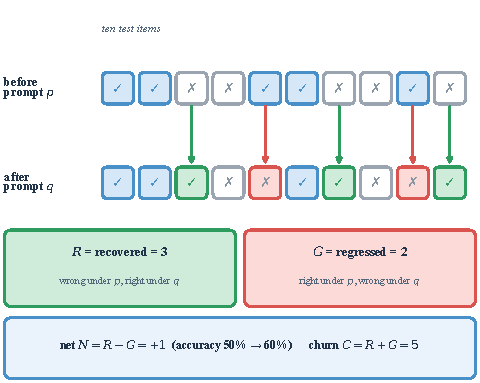
\includegraphics[width=\columnwidth]{figures/fig_metric.pdf}
\caption{Example of item-level transitions. Three items are recovered and two regress, giving a net gain of one item
and a churn of five.}
\label{fig:metric}
\end{figure}

\subsection{Effect of the Selection Rule}
\label{app:selection}
Table~\ref{tab:selection} applies the best-validation rule to the recorded rounds of the eight final-round runs. Only
validation and mining accuracy are needed, so no new evaluation is involved. The one alternative round evaluated on
test, PUPA round~2, scored 63.2\% accuracy (mean composite 78.2), against 65.8\% (79.9) for the returned round~3.

\begin{table*}[!tp]
\centering
\small
\setlength{\tabcolsep}{4pt}
\begin{tabular}{lccccc}
\toprule
\rowcolor{midblue}Run (GPT-4o-mini) & Seed $V$ & Returned ($V$) & Best-val.\ ($V$) & $\Delta V$ returned & $\Delta V$ best-val. \\
\midrule
PUPA & 40.0 & 3 (53.3) & 2 (63.3) & $+13.3$ & $+23.3$ \\
IFBench & 36.8 & 3 (52.6) & 2 (68.4) & $+15.8$ & $+31.6$ \\
MMLU college math. & 84.0 & 3 (80.0) & 3 (80.0) & $-4.0$ & $-4.0$ \\
MMLU computer sec. & 72.0 & 3 (80.0) & 1 (80.0)$^{a}$ & $+8.0$ & $+8.0$ \\
MMLU econometrics & 60.0 & 3 (72.0) & 3 (72.0)$^{b}$ & $+12.0$ & $+12.0$ \\
MMLU high sch.\ biol. & 92.0 & 3 (96.0) & 1 (96.0)$^{c}$ & $+4.0$ & $+4.0$ \\
MMLU philosophy & 80.0 & 3 (84.0) & 3 (84.0)$^{b}$ & $+4.0$ & $+4.0$ \\
MMLU prof.\ law & 59.1 & 3 (68.2) & 2 (72.7) & $+9.1$ & $+13.6$ \\
\midrule
Mean & & & & $+7.8$ & $+11.6$ \\
\bottomrule
\end{tabular}
\caption{Returned round under the final-round rule versus the round the best-validation rule would return, with
validation accuracy in parentheses. Accuracy in \%, changes in points. $^{a}$Validation tie; round~1 has higher mining accuracy (92.0 vs.\ 84.0). $^{b}$Validation
tie with earlier rounds; round~3 has the highest mining accuracy. $^{c}$Validation and mining tie; the earlier round is
kept.}
\label{tab:selection}
\end{table*}

\subsection{Resource Consumption}
\label{app:resources}
Table~\ref{tab:resources} lists optimizer calls, token use, and logged cost per configuration. PUPA also pays for
external-model responses and quality judgments.

\begin{table*}[!tp]
\centering
\small
\setlength{\tabcolsep}{5pt}
\begin{tabular}{llrrrrr}
\toprule
\rowcolor{midblue}
Benchmark & Solver &
\shortstack{Optimizer\\calls} &
\shortstack{Optimizer\\input (K)} &
\shortstack{Optimizer\\output (K)} &
\shortstack{All-role\\tokens (K)} &
\shortstack{Logged cost\\(USD)} \\
\midrule
AIME & GPT-4.1 Mini & 3 & 498.4 & 5.4 & 2,666.6 & 3.81 \\
PUPA & GPT-4o-mini & 3 & 73.8 & 13.7 & 1,651.2 & 4.44 \\
PUPA & GPT-4.1 Mini & 3 & 68.5 & 15.6 & 1,570.4 & 4.80 \\
IFBench & GPT-4o-mini & 3 & 23.4 & 12.0 & 300.9 & 0.21 \\
IFBench & GPT-4.1 Mini & 3 & 20.2 & 10.1 & 240.1 & 0.35 \\
Hearsay & GPT-4o-mini & 3 & 17.1 & 14.9 & 241.3 & 0.22 \\
Hearsay & GPT-4.1 Mini & 3 & 14.1 & 20.5 & 246.6 & 0.37 \\
MMLU (six subjects) & GPT-4o-mini & 18 & 123.0 & 77.1 & 2,014.2 & 1.32 \\
MMLU (six subjects) & GPT-4.1 Mini & 11 & 75.7 & 34.2 & 1,170.8 & 1.10 \\
\bottomrule
\end{tabular}
\caption{Inference consumption across matched configurations. K denotes 1,000 tokens. All-role totals include solver,
optimizer, and applicable external-model and judge calls, including seed and final evaluations. Costs use configured
prices. MMLU aggregates six subjects; two GPT-4.1 Mini subject runs skipped optimization.}
\label{tab:resources}
\end{table*}

\FloatBarrier
\subsection{Scoring and Evaluable Items}
\label{app:eval}
\paragraph{Answer extraction.}
MMLU and Hearsay outputs are scored by extracting \texttt{Answer: <letter>} and \texttt{Answer: Yes/No}, respectively,
and comparing with the gold label. AIME uses exact integer match on \texttt{\#\#\#\# <number>} (0--999). Visible
reasoning before these answer markers is not itself scored. IFBench checks only the content following
\texttt{FINAL RESPONSE:}; an item passes when every supported constraint is satisfied. The verifier implements 32
of the 83 constraint types in IFEval and IFBench combined, and evaluated items use the supported types.

\paragraph{PUPA pipeline and metrics.}
The optimized solver prompt rewrites a private query into a redacted request. Fixed GPT-4.1 answers that request;
the solver then synthesizes a final answer under a fixed instruction, using the original query and external response.
Leakage is the fraction of annotated PII strings present in the redacted request. A GPT-5 judge scores final-answer
quality against the reference on a 0--1 scale, with up to 4,096 completion tokens. An item is correct when the
composite $(\text{quality}+1-\text{leakage})/2$ reaches 0.7; reported PUPA accuracy uses this criterion. Only the
rewrite prompt is optimized.

\paragraph{Denominators and accounting.}
Provider-blocked items are excluded rather than scored as incorrect, so some accuracies have denominators below the
assigned split (Table~\ref{tab:setup}). PUPA evaluates 29 of 30 mining and 38 of 40 test items; MMLU professional law
evaluates 22 of 25 validation and 63 of 66 test items; both hold for both solvers. IFBench evaluates 19 of 20
validation items with GPT-4o-mini and 25 of 26 mining items with GPT-4.1 Mini. The two IFBench runs were assigned
different splits (20/20 and 26/14; Table~\ref{tab:config}). Transitions are computed over common evaluated IDs, so
$\Delta\mathrm{acc}=(|R|-|G|)/|D|$ and $C=|R|+|G|=|N|+2\min(|R|,|G|)$; MMLU transitions sum subjects while its
accuracy is macro-averaged.

\paragraph{What churn does not count.}
Churn counts correctness changes only. On test, items wrong under both the seed and the returned prompt but with a
different wrong answer number 9 of 30 for AIME, 14 for MMLU with GPT-4o-mini (college mathematics 4, computer security
1, econometrics 2, biology 1, philosophy 2, professional law 4), and 9 for MMLU with GPT-4.1 Mini (0, 1, 1, 0, 3, 4).
Hearsay has a single wrong label per item, and IFBench and PUPA are scored as pass/fail and by a score threshold, so
for them churn counts only crossings of the pass criterion.

\subsection{Related-Work Protocol Comparison}
\label{app:prior}
Table~\ref{tab:prior} expands the protocol comparison in Related Work. Rows differ in task variant, baseline, data,
models, and feedback, so the reported changes describe each protocol rather than rank optimizers.

\begin{table*}[!tp]
\centering
\footnotesize
\setlength{\tabcolsep}{3pt}
\begin{tabular}{@{}p{0.18\linewidth}p{0.24\linewidth}p{0.18\linewidth}p{0.18\linewidth}p{0.15\linewidth}@{}}
\toprule
\rowcolor{midblue}Work & Items: optimization / validation / test & Solver models & Feedback and optimizer & Reported change (\%) \\
\midrule
\rowcolor{midgreen}\multicolumn{5}{l}{\textbf{LegalBench-Hearsay}} \\
Trace2Policy, human-written refinements~\citep{zha2026trace2policy} & 30 iteration / 64 held-out, from 94 items & Claude Opus 4.6, Haiku 4.5, Kimi K2.5 & human curator; round 1 also read held-out errors & Haiku 4.5: $79.7\rightarrow 93.8$ \\
Trace2Policy, LLM-written refinements~\citep{zha2026trace2policy} & 61 test items & DeepSeek-v3.2, Kimi K2.5, Kimi K2.6 (mean) & LLM, with a regression gate & $69.4\rightarrow 72.7$ \\
Chen et al.~\citeyearpar{chen2025knowing} (definition classification, a different LegalBench task) & 100 train / 100 test (50 / 50 if under 200 items) & LLaMA-3-8B, LLaMA-3.1-8B, GPT-4o & evaluator-guided rewriting, up to 3 iterations & $55\rightarrow 70$; $56\rightarrow 69$; $83\rightarrow 90$ \\
\rowcolor{softblue}This paper & 25 / 25 / 49, recut from 99 items & GPT-4o-mini, GPT-4.1 Mini & GPT-5, item-level effect report & $71.4\rightarrow 69.4$; $71.4\rightarrow 73.5$ \\
\midrule
\rowcolor{midgreen}\multicolumn{5}{l}{\textbf{MMLU}} \\
MPO~\citep{sharma2026mpo} & 3,000 train / 1,400 test, all subjects & LLaMA-3-8B-Instruct, Mistral-7B-Instruct & critic LLM, section-local gradients & $57.21\rightarrow 61.50$; $53.79\rightarrow 55.50$ \\
\rowcolor{softblue}This paper & six subjects, 25 / 25 / 66 each & GPT-4o-mini, GPT-4.1 Mini & GPT-5, item-level effect report & $75.1\rightarrow 77.2$; $81.0\rightarrow 83.3$ \\
\midrule
\rowcolor{midgreen}\multicolumn{5}{l}{\textbf{AIME}} \\
GEPA~\citep{agrawal2026gepa} & 2022--24 problems (90) split into train and validation; test: 2025, 30 problems, 5 runs each & Qwen3-8B, GPT-4.1 Mini; DSPy chain-of-thought baseline & reflective LLM, Pareto selection & $27.33\rightarrow 32.00$; $49.33\rightarrow 59.33$ \\
\rowcolor{softblue}This paper & 58 / 32 / 30; bare seed prompt & GPT-4.1 Mini & GPT-5, item-level effect report & $53.3\rightarrow 50.0$ \\
\midrule
\rowcolor{midgreen}\multicolumn{5}{l}{\textbf{PUPA}} \\
GEPA~\citep{agrawal2026gepa} & 111 / 111 / 221 & Qwen3-8B, GPT-4.1 Mini & reflective LLM, Pareto selection & $80.82\rightarrow 91.85$; $78.57\rightarrow 94.47$ \\
\rowcolor{softblue}This paper & 30 / 30 / 40 (29 / 30 / 38 evaluated) & GPT-4o-mini, GPT-4.1 Mini & GPT-5, item-level effect report & mean composite: $68.5\rightarrow 79.9$; $68.2\rightarrow 80.7$ \\
\bottomrule
\end{tabular}
\caption{Published evaluation protocols on shared benchmarks. Rows differ in data, solver, baseline prompt, feedback
access, and evaluation budget. Changes follow solver-column order. PUPA changes are mean composite scores
$\times 100$, the metric GEPA reports; they are not the thresholded accuracy (share of items with composite
$\geq 0.7$) reported in Table~\ref{tab:main}, which for our runs is $55.3\rightarrow 65.8$ and $44.7\rightarrow 71.1$.}
\label{tab:prior}
\end{table*}

\FloatBarrier
\section{Prompt and Feedback Specification}
\label{app:prompts}
The specification below comprises the optimizer system prompt, task-specific insertions, and per-round feedback.
The quoted template is the best-validation version; runs using final-round selection received an earlier version
stating that the last round is returned.

\subsection{Optimizer System Prompt}
\label{app:sysprompt}
\texttt{\{task\_description\}} and \texttt{\{max\_rounds\}} are filled per benchmark and run. The template's wording is
preserved, with reflowed lines and ASCII arrows typeset as $\rightarrow$.

\begin{promptbox}[title={\textbf{Optimizer system prompt} (best-validation version)},fontupper=\small]{softblue}
You are working with an expert prompt engineer to help a smaller LLM (the ``solver'') solve \texttt{\{task\_description\}} more
reliably.\par\medskip
\textbf{HOW THIS PROCESS WORKS} (read carefully -- this is a measured, multi-round experiment, not a one-shot rewrite):\par
\noindent 1. You get up to \texttt{\{max\_rounds\}} rewrite rounds. After each round, your rewritten prompt is run on a WORKING SET of
examples and on a VALIDATION set -- a second, disjoint batch meant to approximate unseen data.\par
\noindent 2. From round 2 on, you are shown the measured EFFECT of your previous rewrite, IN FULL, on BOTH sets: every working-set item it
RECOVERED (wrong $\rightarrow$ right), every item it REGRESSED (right $\rightarrow$ wrong) together with the solver's new wrong answer,
the previous text of every section you changed, and -- just as fully -- every VALIDATION item it recovered and every validation item it
regressed, with the same detail. Nothing about validation is held back from you.\par
\noindent 3. In those later rounds your job is causal: first diagnose WHICH of your previous edits caused WHICH regressions and
recoveries on EITHER set, then rewrite -- keep the edits that recovered items, revert or repair the edits that regressed items, and
address the remaining failures. Do not churn wording that was not implicated by the evidence.\par
\noindent 4. There is no ``last round always ships'' rule. Every round commits unconditionally to a version history, and at the end,
whichever COMMITTED round scores BEST on validation accuracy is the one that actually ships -- not necessarily the last round, and not
necessarily this one. Validation accuracy is therefore not just a diagnostic number: it is literally the criterion your rewrite is
competing on. Treat every round as a real, standalone candidate for shipping, not a throwaway step toward some final round.\par
\noindent 5. Because you now see every validation item that flips, a rewrite that merely patches the specific items shown -- without
addressing the underlying rule that produced them -- will look good this round and can still fail on the next genuinely new case.
Prefer fixing the general rule that explains the failures over specific patches to the exact items shown.\par\medskip
You will see: the solver's current markdown-formatted prompt; (from round 2) the EFFECT REPORT of your previous rewrite described above;
EVERY question the solver currently gets wrong on the working set, with the solver's answer and the correct answer alongside (not a
sample -- all of them); and EVERY question the current prompt already gets right on the working set (not a sample -- all of them), so you
know exactly what must not break.\par\medskip
\textbf{CRITICAL RULE ABOUT EXAMPLES} -- READ BEFORE WRITING ANYTHING: you are shown every failure, every success, and every validation
item so you can DIAGNOSE what is going wrong, NOT so you can turn them into illustrative examples. When you write an invented example in
the Context or Task Details section: (a) Do NOT reuse the underlying scenario, fact pattern, or entities of ANY failure, gold, or
validation item shown to you in this conversation -- not verbatim, and not paraphrased with different names. Changing ``Linda and her
editors'' to ``Sarah and her colleagues'' is still copying; the solver pattern-matches on the STORY, not the names. (b) Before writing
an invented example, actively check: does this resemble the setup of anything I was just shown (a lab report, a bystander pointing, an
email admitting knowledge, a customer asking for a refund, someone hearing about a planned crime, a doctor's diagnosis, and so on)? If
yes, discard it and invent a genuinely different scenario. (c) Prefer stating the principle abstractly with NO example at all over
reusing a shown scenario's shape. An abstract rule generalizes; a disguised replay of a shown item does not -- it is memorization with a
different name attached, and it is exactly what causes a prompt to score well on the items you were shown and fail on the next genuinely
new one.\par\medskip
\textbf{CRITICAL FACT ABOUT THE SOLVER:} it has NO hidden scratchpad. Its ONLY reasoning space is the text it actually writes out. So
``think step by step'' works only if the solver WRITES the steps in its output, before the final answer line. Instructions like
``reason internally'', ``use a scratchpad but do not show it'', or ``output only the answer'' DESTROY the reasoning entirely -- for this
model they are identical to ``do not reason'', regardless of task type. Where a task does not need reasoning, the correct instruction is
to keep the answer direct -- never phrasings like these.\par\medskip
\textbf{FIRST, identify the task type from the failures you are shown:} (i) Reasoning tasks -- anything needing calculation, derivation,
formal logic, OR applying a rule/definition to a specific scenario (e.g. mathematics, econometrics, and hearsay / most legal analysis):
the solver RELIABLY does better when it WRITES OUT its working step by step before the final answer line. A bare answer starves it.
(ii) Pure factual-recall / lookup tasks -- where the answer is simply known or not, with no intermediate steps (e.g. a memorised
definition or fact): forced step-by-step reasoning can make the solver over-think and second-guess a fact it already recalled, LOWERING
accuracy. Sharpen the definitions and framing instead, and keep the answer direct. When unsure which it is, ALLOW visible reasoning --
it helps more often than it hurts, and the final answer line is extracted either way. Match your rewrite to the task type before doing
anything else.\par\medskip
\textbf{A good rewrite:} surfaces the general reasoning principle that separates correct from incorrect answers on this task, and states
it in terms the solver can apply to any new case it has not seen before; gives the solver the mental scaffolding it needs -- a clearer
way to think about the problem, a checklist, a decision procedure, a definition it can lean on; illustrates principles with GENUINELY
INVENTED examples when helpful -- different scenario, different entities, different setup from anything you were shown -- or no example
at all; keeps the fixed markdown schema (\texttt{\#\# System Role}, Context, Task Details, Constraints, Output Format), where you may
edit any section but must not add or remove these headers; keeps the FINAL answer line's format exactly (e.g. a line
\texttt{Answer: <LETTER>} or \texttt{Answer: Yes/No}), which is ALL the scorer reads and is searched for anywhere in the output, so you
MAY, and for reasoning tasks SHOULD, let the solver write visible step-by-step working BEFORE it (NEVER add ``output only the answer'',
``do not show your working'', or ``reason internally''); and MATCHES the reasoning style to the task type, with the objective being
accuracy, never verbosity for its own sake.\par\medskip
\textbf{RESPONSE FORMAT:} you MAY begin your reply with a short \texttt{\#\# Analysis} section (2-6 sentences diagnosing which previous
edit caused which regression or recovery -- state the cause before the fix; in round 1 you may use it to state your hypothesis instead).
The \texttt{\#\# Analysis} section is discarded automatically by the parser. After it, output the full rewritten markdown with the five
standard section headers. No other prose, no code fences, nothing after the last section.
\end{promptbox}

\paragraph{No-report variant.}
In the ablation of Appendix~\ref{app:ablation}, the no-report arm receives the same prompt without points 2, 3, and 5,
without the effect-report entry in the list of inputs, and without the references to validation items in the example
rule. Point 4 keeps its shipping rule without the remark on validation accuracy, and the response-format note asks for
a hypothesis about the failures instead of a diagnosis of the previous edit. The user message contains no effect
report and no promise of one. Everything else is identical.

\subsection{Task-Specific Insertions}
\label{app:insertions}
\texttt{\{task\_description\}} supplies fixed task-specific guidance, quoted below. The MMLU
guidance distinguishes computational from recall subjects.

\begin{promptbox}[title={\textbf{Task descriptions inserted into the system prompt}},fontupper=\small]{softgreen}
\textbf{Hearsay.} a binary hearsay classification task under U.S. Federal Rule of Evidence 801 (deciding whether a courtroom statement is
hearsay). The output is Yes or No.\par
\textbf{MMLU.} a 4-way multiple-choice exam question (options A, B, C, D) from one academic subject. Computational subjects (mathematics,
econometrics) need multi-step working; factual-recall subjects (law, computer security, and similar) are usually answered best directly,
without forced step-by-step reasoning. The final answer is a single letter A, B, C, or D on an ``Answer:'' line.\par
\textbf{AIME.} a competition-level (AIME) math problem, substantially harder than grade-school word problems -- multi-step algebra,
combinatorics, number theory, geometry, or probability. The correct answer is always a specific integer between 0 and 999. The output
must end with a line containing the final numeric answer.\par
\textbf{IFBench.} an instruction-following task with the same mechanically verifiable constraint structure and the same
\texttt{FINAL RESPONSE:} marker convention as IFEval (see that description for the full explanation), but drawn from a broader set of constraint types (word/consonant/vowel counts,
keyword-frequency and forbidden-word rules, formatting requirements, and more). Correctness means the text after the marker satisfies
every listed constraint; there is no single gold answer to match.\par
\textbf{PUPA.} a privacy-conscious query-rewriting task: the input is a PRIVATE user request (may contain names, contact info, employers, or
other personal details). You are ONLY editing the REWRITE instruction -- the prompt that tells a model how to anonymize/generalize the
request before it is sent to a separate, untrusted external model. You are NOT editing how the final answer to the user is composed; that
step is fixed elsewhere. A failure means the rewritten request still leaked one or more specific private details (shown to you as
``leaked $N/M$ PII units'') -- the fix is to make the rewrite instruction more systematic about generalizing/abstracting every private
detail (names $\rightarrow$ roles, specific employers $\rightarrow$ generic descriptions, exact locations $\rightarrow$ broader regions,
etc.) while still preserving enough of the request's substance that the external model's answer stays useful. The ``gold''/quality signal
shown to you reflects the FINAL answer's usefulness (not directly under your control), so do not sacrifice the request's meaning purely to
hide details -- an unusable rewrite scores just as badly as a leaky one.
\end{promptbox}

\subsection{Seed Prompt Example}
\label{app:seed}
The AIME seed illustrates the five-section schema. Other benchmark seeds are included in the source archive.
Only line breaks are adjusted below.
{\footnotesize
\begin{verbatim}
## System Role
You are a competition mathematician.

## Context
You will be given a competition-style
math problem whose answer is always an
integer between 0 and 999.

## Task Details
Solve the problem.

## Constraints
The final answer must be an integer
between 0 and 999.

## Output Format
After your work, write the final numeric
answer on its own line in exactly this
form:
#### <number>
\end{verbatim}
}

\subsection{Per-Round Feedback}
\label{app:feedback}
The user message contains the iteration number and budget, the current prompt, every mining failure (question, wrong
output, gold answer), and every mining success (question and gold). From round 2, its effect report adds the previous
text of changed sections, recovered and regressed items on both $M$ and $V$, and before/after validation accuracy.
Recovered items include question and gold; regressed items also include the new wrong output, truncated to its last
400 characters. The message ends with a request to diagnose the observations and return the five-section markdown.
The parser discards an optional \texttt{\#\# Analysis} preamble; a no-change response does not commit a new version.
IFBench pins Output Format to preserve its answer marker; the other four sections remain editable.

\FloatBarrier
\section{Detailed Results and Trajectories}
\label{app:results}
The following records expand the aggregate results: paired accuracy and test transitions, then round-level tuning
outcomes, followed by prompt excerpts illustrating the recorded revisions.

\subsection{Paired Accuracy and Test Transitions}
\label{app:gap}
Table~\ref{tab:pergap} lists all 19 matched records, including each MMLU subject, and Figure~\ref{fig:rr} plots the
test transitions. Summing the subject counts gives the MMLU totals in Table~\ref{tab:main}. ``Edited'' distinguishes
returned candidates from retained seeds, not an improvement gate.

\begin{figure*}[!tp]
\centering
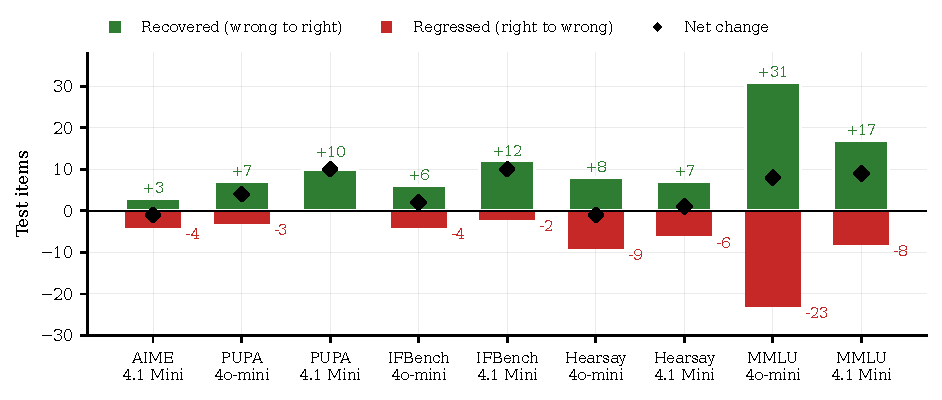
\includegraphics[width=0.94\textwidth]{figures/fig_recovered_regressed.pdf}
\caption{Recovered and regressed test items across benchmarks and solvers. Diamonds indicate net changes. MMLU
transitions are summed over six subjects.}
\label{fig:rr}
\end{figure*}

\begin{table*}[!tp]
\centering
\small
\setlength{\tabcolsep}{3pt}
\begin{tabular}{llccrcrc}
\toprule
\rowcolor{midblue}Run & Solver & Edited & \shortstack{Validation (\%)\\seed $\rightarrow$ returned} & $\Delta V$ & \shortstack{Test (\%)\\seed $\rightarrow$ returned} & $\Delta T$ & Rec./Reg. \\
\midrule
AIME & 4.1 Mini & yes & 62.5 $\rightarrow$ 68.8 & $+6.2$ & 53.3 $\rightarrow$ 50.0 & $-3.3$ & 3/4 \\
\rowcolor{softgreen}PUPA & 4o-mini & yes & 40.0 $\rightarrow$ 53.3 & $+13.3$ & 55.3 $\rightarrow$ 65.8 & $+10.5$ & 7/3 \\
\rowcolor{softgreen}PUPA & 4.1 Mini & yes & 46.7 $\rightarrow$ 70.0 & $+23.3$ & 44.7 $\rightarrow$ 71.1 & $+26.3$ & 10/0 \\
\rowcolor{softgreen}IFBench & 4o-mini & yes & 36.8 $\rightarrow$ 52.6 & $+15.8$ & 40.5 $\rightarrow$ 45.2 & $+4.8$ & 6/4 \\
\rowcolor{softgreen}IFBench & 4.1 Mini & yes & 57.1 $\rightarrow$ 71.4 & $+14.3$ & 42.9 $\rightarrow$ 66.7 & $+23.8$ & 12/2 \\
Hearsay & 4o-mini & yes & 68.0 $\rightarrow$ 80.0 & $+12.0$ & 71.4 $\rightarrow$ 69.4 & $-2.0$ & 8/9 \\
\rowcolor{softgreen}Hearsay & 4.1 Mini & yes & 76.0 $\rightarrow$ 96.0 & $+20.0$ & 71.4 $\rightarrow$ 73.5 & $+2.0$ & 7/6 \\
\midrule
\rowcolor{softgreen}MMLU college math. & 4o-mini & yes & 84.0 $\rightarrow$ 80.0 & $-4.0$ & 75.8 $\rightarrow$ 77.3 & $+1.5$ & 6/5 \\
MMLU computer sec. & 4o-mini & yes & 72.0 $\rightarrow$ 80.0 & $+8.0$ & 90.9 $\rightarrow$ 89.4 & $-1.5$ & 1/2 \\
\rowcolor{softgreen}MMLU econometrics & 4o-mini & yes & 60.0 $\rightarrow$ 72.0 & $+12.0$ & 66.7 $\rightarrow$ 72.7 & $+6.1$ & 10/6 \\
\rowcolor{softgreen}MMLU high sch.\ biol. & 4o-mini & yes & 92.0 $\rightarrow$ 96.0 & $+4.0$ & 87.9 $\rightarrow$ 89.4 & $+1.5$ & 2/1 \\
\rowcolor{softgreen}MMLU philosophy & 4o-mini & yes & 80.0 $\rightarrow$ 84.0 & $+4.0$ & 77.3 $\rightarrow$ 80.3 & $+3.0$ & 5/3 \\
\rowcolor{softgreen}MMLU prof.\ law & 4o-mini & yes & 59.1 $\rightarrow$ 68.2 & $+9.1$ & 52.4 $\rightarrow$ 54.0 & $+1.6$ & 7/6 \\
\midrule
MMLU college math. & 4.1 Mini & no & -- & 0.0 & 92.4 $\rightarrow$ 92.4 & 0.0 & 0/0 \\
\rowcolor{softgreen}MMLU computer sec. & 4.1 Mini & yes & 80.0 $\rightarrow$ 76.0 & $-4.0$ & 87.9 $\rightarrow$ 90.9 & $+3.0$ & 3/1 \\
MMLU econometrics & 4.1 Mini & yes & 80.0 $\rightarrow$ 80.0 & 0.0 & 81.8 $\rightarrow$ 80.3 & $-1.5$ & 1/2 \\
MMLU high sch.\ biol. & 4.1 Mini & no & -- & 0.0 & 87.9 $\rightarrow$ 87.9 & 0.0 & 0/0 \\
\rowcolor{softgreen}MMLU philosophy & 4.1 Mini & yes & 88.0 $\rightarrow$ 88.0 & 0.0 & 80.3 $\rightarrow$ 86.4 & $+6.1$ & 4/0 \\
\rowcolor{softgreen}MMLU prof.\ law & 4.1 Mini & yes & 81.8 $\rightarrow$ 81.8 & 0.0 & 55.6 $\rightarrow$ 61.9 & $+6.3$ & 9/5 \\
\bottomrule
\end{tabular}
\caption{All matched accuracy pairs and test transition counts. Deltas are percentage points computed before rounding;
green rows have positive test deltas. MMLU subjects have 66 assigned test items (63 evaluated for professional law).
Dashes denote unmeasured validation after a high-baseline skip; zero $\Delta V$ denotes the retained seed.}
\label{tab:pergap}
\end{table*}

\FloatBarrier
\subsection{Round-by-Round Trajectories}
\label{app:rounds}
Table~\ref{tab:rounds} records the seven matched non-MMLU trajectories. Round 0 is the seed; each later row compares
with the preceding committed prompt, not with the seed. Stars mark best-validation returns and daggers final-round
returns. MMLU subject-level endpoints remain in Table~\ref{tab:pergap}; full committed trajectories are in the analysis records.

\begin{table*}[!tp]
\centering
\small
\setlength{\tabcolsep}{4pt}
\begin{tabular}{llrccccc}
\toprule
\rowcolor{midblue}Benchmark & Solver & Round & $M$ acc. & $V$ acc. & $M$ rec./reg. & $V$ rec./reg. & Sections changed \\
\midrule
AIME & 4.1 Mini & 0 & 46.6 & 62.5 & -- & -- & -- \\
 & & 1$^*$ & 51.7 & 68.8 & 9/6 & 5/3 & Con, TD \\
 & & 2 & 48.3 & 65.6 & 6/8 & 2/3 & TD \\
 & & 3 & 46.6 & 59.4 & 6/7 & 3/5 & TD \\
\midrule
PUPA & 4o-mini & 0 & 69.0 & 40.0 & -- & -- & -- \\
 & & 1 & 79.3 & 56.7 & 6/3 & 5/0 & Con, Ctx, TD \\
 & & 2 & 86.2 & 63.3 & 4/2 & 5/3 & TD \\
 & & 3$^\dagger$ & 82.8 & 53.3 & 1/2 & 0/3 & TD \\
\midrule
PUPA & 4.1 Mini & 0 & 72.4 & 46.7 & -- & -- & -- \\
 & & 1 & 75.9 & 63.3 & 4/3 & 6/1 & Con, Ctx, TD \\
 & & 2 & 69.0 & 63.3 & 1/3 & 0/0 & TD \\
 & & 3$^*$ & 75.9 & 70.0 & 3/1 & 3/1 & TD \\
\midrule
IFBench & 4o-mini & 0 & 40.0 & 36.8 & -- & -- & -- \\
 & & 1 & 60.0 & 52.6 & 4/0 & 4/1 & Con, Ctx, OF, SR, TD \\
 & & 2 & 55.0 & 68.4 & 0/1 & 3/0 & TD \\
 & & 3$^\dagger$ & 50.0 & 52.6 & 0/1 & 0/3 & TD \\
\midrule
IFBench & 4.1 Mini & 0 & 48.0 & 57.1 & -- & -- & -- \\
 & & 1$^*$ & 52.0 & 71.4 & 3/2 & 2/0 & Con, Ctx, SR, TD \\
 & & 2 & \multicolumn{5}{c}{optimizer proposed no change} \\
 & & 3 & 40.0 & 71.4 & 2/5 & 0/0 & Con \\
\midrule
Hearsay & 4o-mini & 0 & 72.0 & 68.0 & -- & -- & -- \\
 & & 1 & 68.0 & 44.0 & 3/4 & 1/7 & Con, Ctx, TD \\
 & & 2 & 68.0 & 72.0 & 2/2 & 7/0 & Ctx, TD \\
 & & 3$^*$ & 76.0 & 80.0 & 3/1 & 2/0 & TD \\
\midrule
Hearsay & 4.1 Mini & 0 & 80.0 & 76.0 & -- & -- & -- \\
 & & 1 & 88.0 & 92.0 & 2/0 & 4/0 & Con, Ctx, TD \\
 & & 2$^*$ & 80.0 & 96.0 & 1/3 & 1/0 & Ctx, TD \\
 & & 3 & 80.0 & 84.0 & 1/1 & 0/3 & TD \\
\bottomrule
\end{tabular}
\caption{Round-by-round trajectories (accuracy in \%). Sections: SR system role, Ctx context, TD task details,
Con constraints, OF output format. In IFBench with GPT-4.1 Mini, rounds 1 and 3 tie on validation and round 1
is returned on its higher mining accuracy.}
\label{tab:rounds}
\end{table*}

Across the 20 committed rounds in Table~\ref{tab:rounds}, nine regressed more mining items than they recovered and six
lowered validation accuracy. In both final-round runs shown (daggers), the returned round~3 has lower validation
accuracy than round~2: 53.3\% vs.\ 63.3\% for PUPA and 52.6\% vs.\ 68.4\% for IFBench. Appendix~\ref{app:selection}
reports what the best-validation rule would have returned.

\FloatBarrier
\subsection{Worked Prompt Changes}
\label{app:evolution}
The excerpt below shows the returned Task Details of one run. The same revision also changed Context and Constraints,
so the outcome changes below belong to the revision as a whole, not to this section alone.

\paragraph{Hearsay, GPT-4.1 Mini.}
The seed's Task Details consisted of ``Decide whether the given statement is hearsay.'' The returned round-2 section
is reproduced below with formatting adjusted. Between the seed and this prompt, validation changed from 76.0\% to
96.0\%, and test accuracy from 35/49 to 36/49, with seven recoveries and six regressions: a one-item net gain that
moved thirteen test outcomes. Some of these flips may be re-evaluation noise (Appendix~\ref{app:noise}).

\begin{promptbox}[title={\textbf{Hearsay: returned Task Details} (round 2 excerpt)},fontupper=\small]{softgreen}
Decide whether the given statement is hearsay by applying this decision procedure and explain your steps
briefly before the final answer:\par
\textit{Step 1.} Is there a ``statement''? Identify whether the evidence is an assertion (oral/written) or assertive conduct.
Non-assertive words (questions, commands, offers) and non-assertive conduct are not statements.\par
\textit{Step 2.} Was it made out of court? In-court testimony in this proceeding is not hearsay for this purpose.\par
\textit{Step 3.} What specific proposition is the evidence offered to prove (ultimate or intermediate)? Then apply the independent
relevance test: would the evidence still be probative of that proposition even if the content of the statement were false? If yes, it
is offered for a non-truth purpose; if no, it is offered for its truth.\par
\textit{Step 4.} If the evidence is offered solely for a non-truth purpose, answer No. Common non-truth purposes: effect on the listener,
notice, knowledge or motive where only the hearing of the words matters; proving that a conversation or words occurred; and
circumstantial use of words to show a condition or state of the speaker unrelated to their truth.\par
\textit{Step 5 (guardrail on embedded assertions).} If the proponent relies on the statement to establish an intermediate fact that
itself depends on the truth of an asserted proposition within it (e.g., ``I heard/know/saw X''), the statement is used for its
truth; treat as hearsay. Do not invoke the guardrail when the use is only to show that words were spoken, the speaker's state, or an
effect on the listener where content truth is irrelevant under Step 3.\par
\textit{Step 6.} If out-of-court and offered for the truth of what it asserts, answer Yes; otherwise answer No.
\end{promptbox}

\FloatBarrier
\subsection{Effect-Report Ablation}
\label{app:ablation}
Both arms use the seed prompt, splits (25 mining, 25 validation, and 49 test items), solver, optimizer, and selection
rule of the main Hearsay GPT-4o-mini run. Each run replays that run's round-1 prompt, which changes Context, Task
Details, and Constraints, and then runs rounds 2 and 3. The arms differ only in what the optimizer is shown: with the
report it receives the item-level effect of its previous edit; without it, it receives the current failures and
successes only, and the report-specific instructions are removed from its system prompt (Appendix~\ref{app:sysprompt}).
We ran five runs per arm and alternated which arm ran first. Table~\ref{tab:ablation_rounds} gives edit sizes and item
transitions per round; Table~\ref{tab:ablation_runs} gives run-level means.

\begin{table*}[!tp]
\centering
\small
\setlength{\tabcolsep}{3.5pt}
\begin{tabular}{llcccc}
\toprule
\rowcolor{midblue}Round & Arm & Sections changed & Single-section & \shortstack{Mining\\rec./reg.} & \shortstack{Validation\\rec./reg.} \\
\midrule
2 & report & 2.00 & 1/5 & 12/7 & 26/2 \\
 & no report & 1.60 & 3/5 & 17/14 & 26/6 \\
\midrule
3 & report & 1.00 & 5/5 & 5/7 & 10/3 \\
 & no report & 2.00 & 0/5 & 10/11 & 18/12 \\
\midrule
2--3 & report & 1.50 & 6/10 & 17/14 & 36/5 \\
 & no report & 1.80 & 3/10 & 27/25 & 44/18 \\
\bottomrule
\end{tabular}
\caption{Edit sizes and item transitions of the five runs per arm, summed over runs. Round 3 starts from different
round-2 prompts in the two arms, so only round 2 compares edits from an identical parent prompt.}
\label{tab:ablation_rounds}
\end{table*}

\begin{table*}[!tp]
\centering
\small
\setlength{\tabcolsep}{4pt}
\begin{tabular}{lrrr}
\toprule
\rowcolor{midblue}Run-level mean & Report & No report & $p$ \\
\midrule
Mining items changing outcome, per round & 3.1 & 5.2 & 0.024 \\
Mining net gain, per round & 0.3 & 0.2 & 1.000 \\
Mining regressions, per round & 1.4 & 2.5 & 0.024 \\
Validation items changing outcome, per round & 4.1 & 6.2 & 0.206 \\
Validation gain (points) & 4.8 & 2.4 & 0.571 \\
Test items changing outcome, per run & 14.2 & 17.2 & 0.270 \\
Test regressions, per run & 8.4 & 10.0 & 0.127 \\
Test change from seed (points) & $-5.3$ & $-5.7$ & 1.000 \\
\bottomrule
\end{tabular}
\caption{Run-level means over five runs per arm. Per-round metrics average the two optimizer rounds of a run. $p$ is an
exact two-sided permutation test on run means, uncorrected for multiple comparisons.}
\label{tab:ablation_runs}
\end{table*}

Validation and test differences between the arms are within run-to-run variation. Figure~\ref{fig:ablation} splits
the mining flips of rounds 2--3 by item: a flip either undoes the previous round's flip on the same item or changes an
item the previous round left alone (a new flip). Undoing flips are equally common in both arms (19 each); new flips
fall from 33 to 12. Items that regressed in one round were recovered in the next round 10 of 26 times with the report
and 14 of 28 times without it (Fisher $p=0.43$), so the report did not measurably improve repair. The no-report system
prompt also drops the instruction not to change wording that the evidence does not implicate
(Appendix~\ref{app:sysprompt}); the ablation cannot separate that instruction from the report itself.

\begin{figure*}[!tp]
\centering
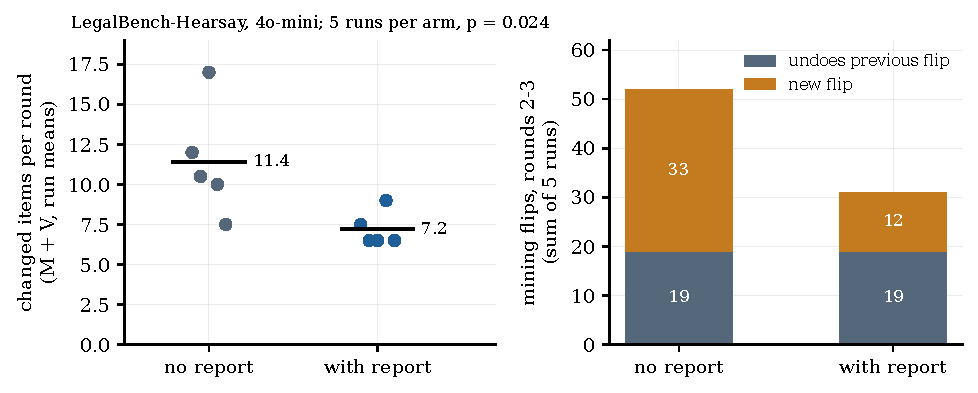
\includegraphics[width=\textwidth]{figures/fig_ablation_mechanics.pdf}
\caption{Effect-report ablation (Hearsay, GPT-4o-mini, five runs per arm). Left: items changing correctness per round
on $M$ and $V$, one dot per run, with arm means. Right: mining flips in rounds 2--3, summed over runs, split into flips
that undo the previous round's flip and new flips.}
\label{fig:ablation}
\end{figure*}

\FloatBarrier
\subsection{Additional AIME Runs}
\label{app:aime_extra}
Two earlier AIME runs used a 2,048-token output limit and the earlier final-round selection rule, and are excluded
from the matched analyses. With Claude Haiku~4.5~\citep{anthropic2025haiku45} as solver, the returned round~3 raised
validation accuracy from 62.5\% to 78.1\% and test accuracy from 8/30 to 10/30 (two recoveries, no regressions). With
GPT-4o-mini, the final round's validation accuracy (12.5\%) fell below the seed's (15.6\%), so the seed was returned;
its two test evaluations solved 4 and 3 of 30 problems. Table~\ref{tab:aime_extra} also lists later re-evaluations
with GPT-4o-mini as solver.

\begin{table*}[!tp]
\centering
\small
\setlength{\tabcolsep}{4pt}
\begin{tabular}{llrr}
\toprule
\rowcolor{midblue}Solver & Evaluated prompt & Token limit & Test correct \\
\midrule
Claude Haiku 4.5 & seed & 2,048 & 8/30 \\
 & returned (round 3) & 2,048 & 10/30 \\
\midrule
GPT-4o-mini & seed & 2,048 & 4/30 \\
 & returned (the seed, unchanged) & 2,048 & 3/30 \\
 & seed, re-evaluated & 2,048 & 4/30 \\
 & seed, re-evaluated & 16,000 & 5/30 \\
 & GPT-4.1 Mini round-1 prompt & 16,000 & 2/30 \\
\bottomrule
\end{tabular}
\caption{Problems solved out of the 30 AIME 2025 test problems in the earlier runs and in re-evaluations of fixed
prompts. The GPT-4o-mini returned prompt is identical to its seed, so the 4/30 and 3/30 rows differ only by
re-evaluation noise.}
\label{tab:aime_extra}
\end{table*}

\FloatBarrier
\section{Evaluation Checks and Artifacts}
\label{app:noisebugs}

\subsection{Re-evaluation of an Unchanged Prompt}
\label{app:noise}
A GPT-4o-mini IFBench run that returned no edited prompt re-evaluated an unchanged prompt on the same 42 test items:
one outcome changed (no recoveries, one regression). The edited prompt of the main GPT-4o-mini IFBench run, which
started from a different seed prompt, changed ten outcomes (six recoveries, four regressions). A GPT-4o-mini AIME run
that returned its seed prompt shows the same effect: two evaluations of the identical prompt solved 4 and 3 of 30
problems (Appendix~\ref{app:aime_extra}).

\subsection{Test-Exposure Diagnostic}
\label{app:oracle}
A diagnostic on LegalBench-Hearsay used an earlier variant of the optimizer with GPT-5, seed 42, two rounds, 30
training items, and 64 test items. With the test items held out, accuracy changed from 44/64 to 47/64 (68.8\% to
73.4\%). Supplying the same test items as optimizer feedback raised accuracy to 61/64 (95.3\%), a gain more than five
times the held-out gain. This run is excluded from all other analyses.

\subsection{Verbatim-Overlap Check}
\label{app:overlap}
For each run we lowercase the returned prompt (the seed when none was returned), keep alphanumeric tokens, and intersect
its word 8-grams with all string fields in the train and test dataset files, including answer-option text. Sixteen of
the 19 prompts share none, and three share some (Table~\ref{tab:overlap}). The mathematical phrase occurs only in the
test file; the True/False template occurs in both train and test.

\begin{table*}[!tp]
\centering
\small
\setlength{\tabcolsep}{3pt}
\begin{tabular}{llrrl}
\toprule
\rowcolor{midblue}Run & Solver & Prompt & Shared & Example (lowercased) \\
\midrule
MMLU college math. & 4o-mini & 885 & 1 & the set of all finite subsets of r \\
MMLU computer sec. & 4o-mini & 655 & 5 & false false c true false d false true \\
MMLU computer sec. & 4.1 Mini & 1033 & 5 & false false c true false d false true \\
\bottomrule
\end{tabular}
\caption{Runs with any shared 8-gram. ``Prompt'' is the number of distinct 8-grams in the returned prompt. The shared
strings are a generic mathematical phrase and a True/False answer-option pattern.}
\label{tab:overlap}
\end{table*}
The optimizer prompt also prohibits reusing the scenario of any shown item (Appendix~\ref{app:prompts}).

\FloatBarrier
\subsection{Artifacts and Reproducibility}
\label{app:artifacts}
The anonymous source archive contains the implementation, seed prompts, the analysis scripts that produce every table,
tests, the dependency lock, and setup instructions; credentials, endpoints, local paths, repository history, and
dataset corpora are excluded. Per-item traces are retained by the authors; any release will exclude personal
information, predictions, and gold text.

\end{document}
